\subsection{Session page}
To create a session the user must first reach the Sessions component, which can be accessed by clicking on the “Sessions” button on the navbar. The session page will have the URL /admin/sessions. A session cannot be created until both a course and a question are present in the database. Therefore, the user will have to visit both the dashboard and the question page first, before accessing the session page. In the figure \ref{fig:sessionPage} shows the session page, in this figure a session has already been created called “Test Økt”. Since there is a session in the database that has a few questions. The Session component is visible in the Sessions component on the right side of the page. If there are no sessions for the chosen course, then only the Sessions component will be displayed on the page. Although if this is the case, then the Sessions component will not have any sessions in the list.
\\[11pt]
The Session component contains a search bar and a select box identical to the ones in the question page. The component also contains a list that will include all the current sessions created for the chosen subject. Just like in the list on the question page, the list on the session page will send a socket emit message to the server in order to keep its session list up to date. The list will be updated whenever the Session component is loaded, a new session is created or whenever the chosen course is changed. Once the Session component is visible, the information displayed on the component will vary depending on the current question being selected. The user can easily change between the available sessions and their questions by clicking on their name. On figure \ref{fig:sessionPage} you can see that the session “Test Økt” has opened the question “Text Question”. 
\\[11pt]
The information displayed on the Session component comes from a component by the name DisplayQuestion. The DisplayQuestion is a component that is used whenever an admin is going to watch question information in the same style as in an active session. Essentially the component is used on the session page and on the user profile page. The DisplayQuestion component uses a vue card, which makes it easier to toggle between showing the question information and the question's solution.  The DisplayQuestion will contain components for solution and answer for each question type, but only one of these components will be used at a time. The DisplayQuestion component has to accommodate for the fact that some of the question types require the GraphDrawer to visually display their solution object. This component will always display what type of question the shown question is. This is done so that the user will know what type of question the question is. This is done to avoid confusing the different question types, as some of the question types have similar set up for the GraphDrawer.
\begin{figure}[H]
	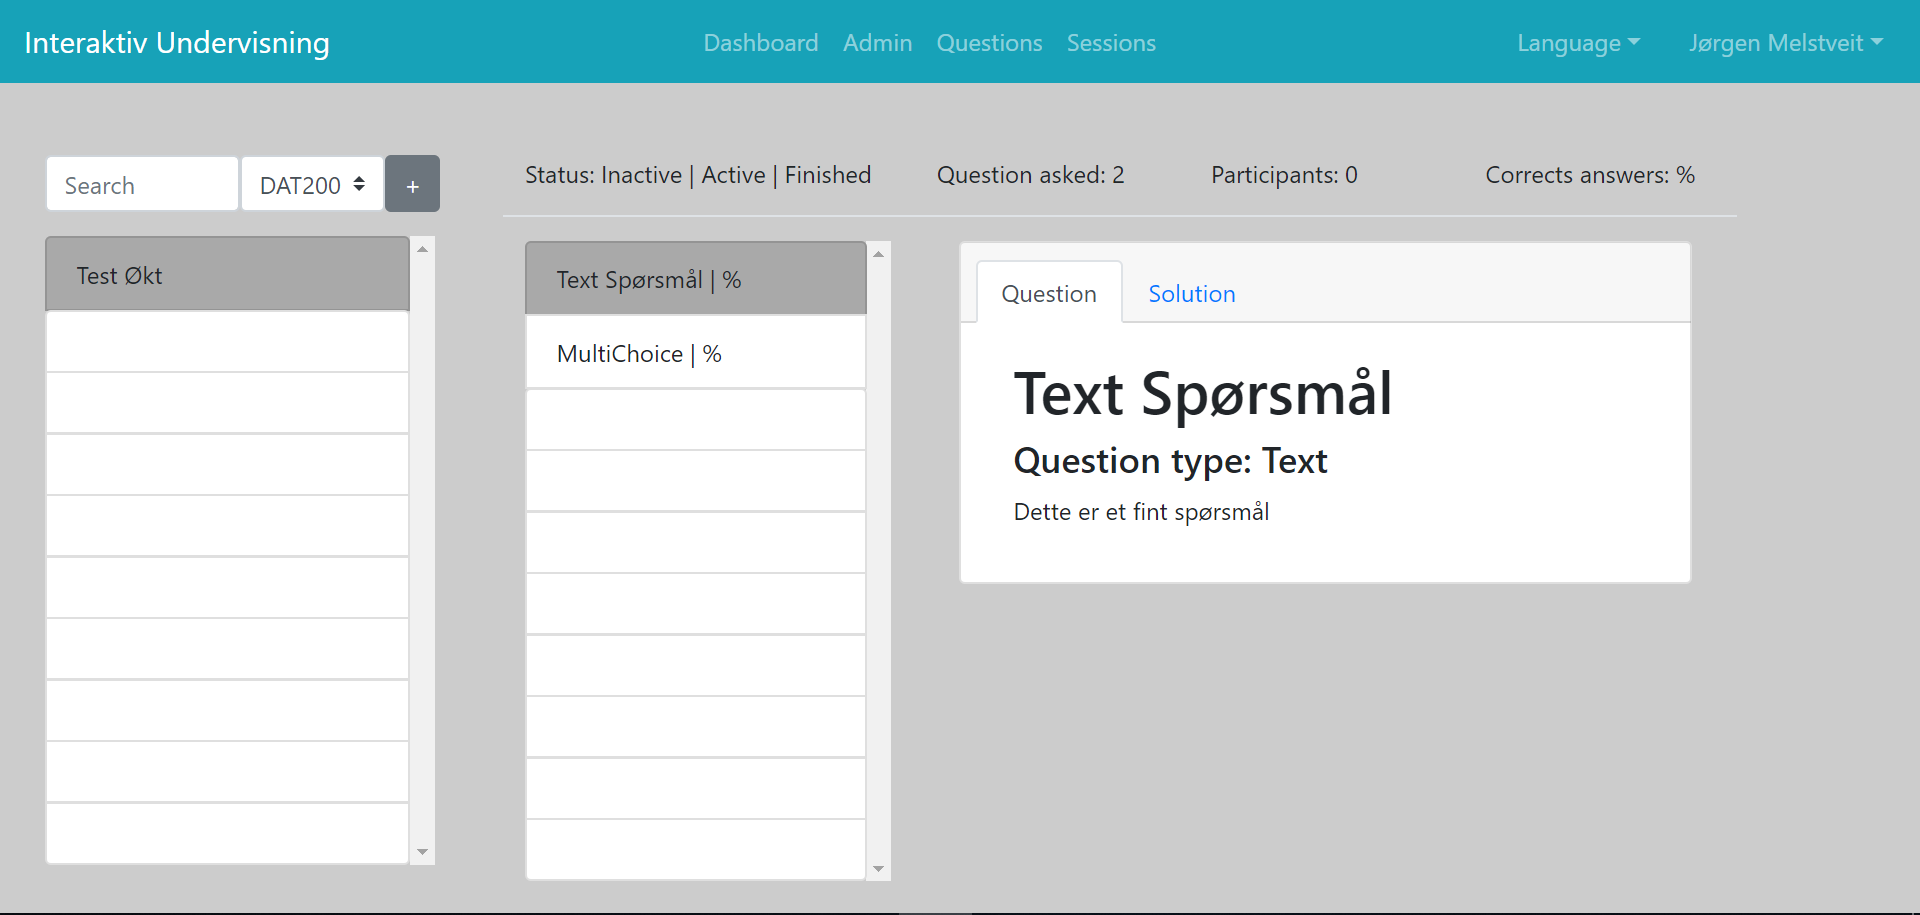
\includegraphics[width=0.80\linewidth]{sessionPage}
	\caption{This figure display the session page. In the image the user is currently checking out the session Test Økt. The Session and DisplayQuestion components are both visible to the right of the image. Currently the Text Spørsmål is selected and the DisplayQuestion is showing its basic information. Such as the title, description and question type.}
	\label{fig:sessionPage}
\end{figure}
Whenever the user wants to create a new session the user must simply click on the button labelled with a “+”. Once this is done, a component EditSession will appear. This component will display all the available question of the chosen course using a vue modal. Similar to the EditQuestion component, the EditSession component has a data object called newSession. This object should have all the values needed for the server to add a new session to the database. The current course should have already been chosen at this point, therefore the course variable in the newSession object should already have been assigned with this course value. This value is used by EditSession component whenever it sends a socket emit to the server, asking the server for all the questions in the given course. The EditSession component will allow the user to give the session a title and add a question to the session. Once a user has clicked on one of the questions, the question will be added to the questions array in the newSession object. The content of the questions array is displayed on the EditSession component under the previous list, and it will react on any changes done to the array. This is noticeable in the figure \ref{fig:editSessionComponent}, where you can see the Text Question has been added to the list under the questions list. Once a question is visible in this way, it means the question will be part of the newly created session. Of course, nothing is stored on the server until the user has clicked on the button with the label “Ok”. When the button is pressed the EditQuestion will send a socket emit with the newSession object to the server. The server collects the objects and the information is used to insert a new session into the Session database table. Afterwards all the questions in the questions array will be linked to the session in another database table in between the Session and Questions tables called the SessionsHasQuestion. Finally, all the questions will have their status be changed to active. This is done so that the questions in the session no longer can be deleted in the questions list. When everything is done the server will send a emit response back to the client. The EditSession component should be closed and the Sessions component will react to the emit response by sending a new socket emit back to the server, in order to update its session list. Once the server respond with the updated session content, the list on the Session component should include the newly created session.  
\begin{figure}[H]
	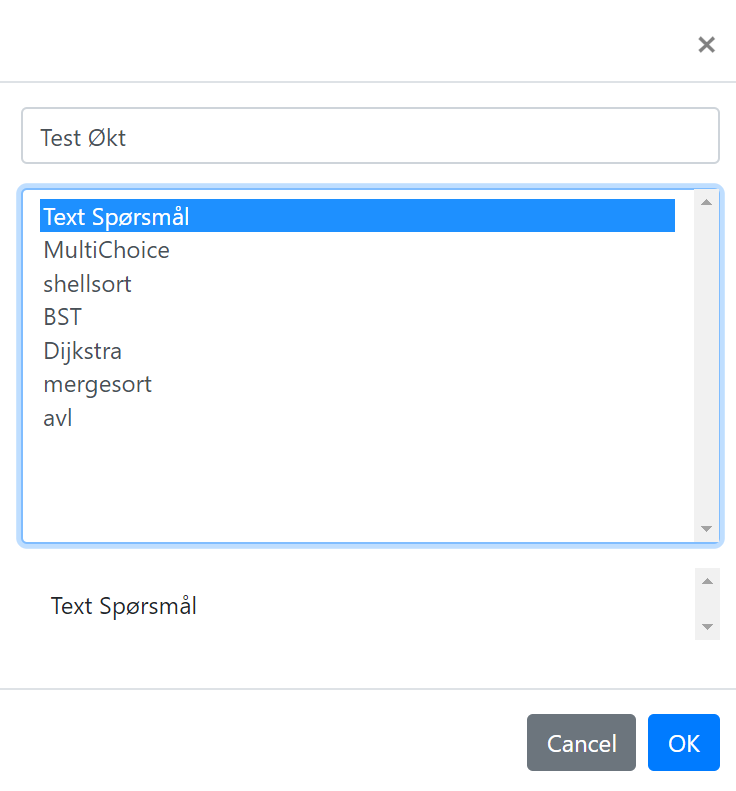
\includegraphics[width=0.80\linewidth]{createANewSession}
	\caption{This figure displays an image of the EditSession component. In the image the user is planning on creating a new session by the name of Text Økt. The image also shows the user having clicked on the Text Spørsmål, which now have been added to the list at the bottom of the page.}
	\label{fig:editSessionComponent}
\end{figure}
